
\chapter{Results and Analysis}
\label{chap:results_analysis}

\section{Simulation Environment Configuration}
\label{sec:simulation_env_config}

The evaluation used the Thapathali SUMO network prepared from OpenStreetMap geometry and OD-based traffic demand. As shown in Figure \ref{fig:simulation_environment}, the simulation includes the Maitighar, Kupondole, Tripureshwor, and Maternity approaches with their lane layout and signal placement. Vehicle classes were represented using PCU factors, and the traffic demand was generated by the allocation process described in Chapter 5. The DQN agent was trained for 300 episodes, with exploration decaying from 1.0 to 0.01, and used the Max-Pressure based reward function described earlier.

\begin{figure}[H]
    \centering
    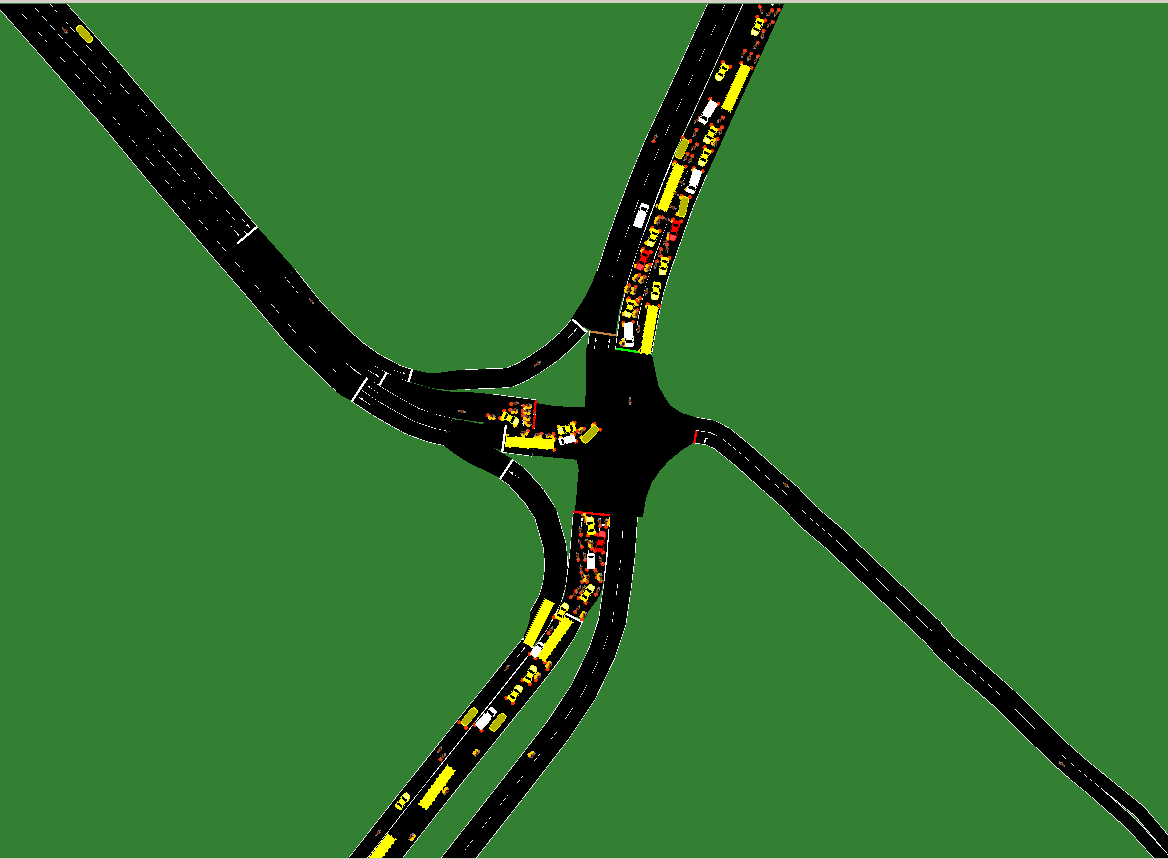
\includegraphics[width=\textwidth]{src/images/figures/simulation_enviroment.png}
    \caption{SUMO Simulation Environment of Thapathali Intersection}
    \label{fig:simulation_environment}
\end{figure}

\section{Training Convergence and Learning Trajectory}
\label{sec:training_convergence}

Figure \ref{fig:reward_function} shows the episode reward and epsilon
decay over 300 training episodes. The first 50 episodes are noisy because
the agent is still exploring; rewards stayed roughly between $\sim$5,500
and $\sim$6,000. After exploration decreased, the moving average began to
improve. By episode 300, it reached 3,395.8 from approximately
$\sim$5,300.

The reward curve suggests that the agent learned a more useful
phase-selection pattern. It is not enough by itself, however, so the
final policy is evaluated using traffic metrics in the following
sections.

\begin{figure}[H]
    \centering
    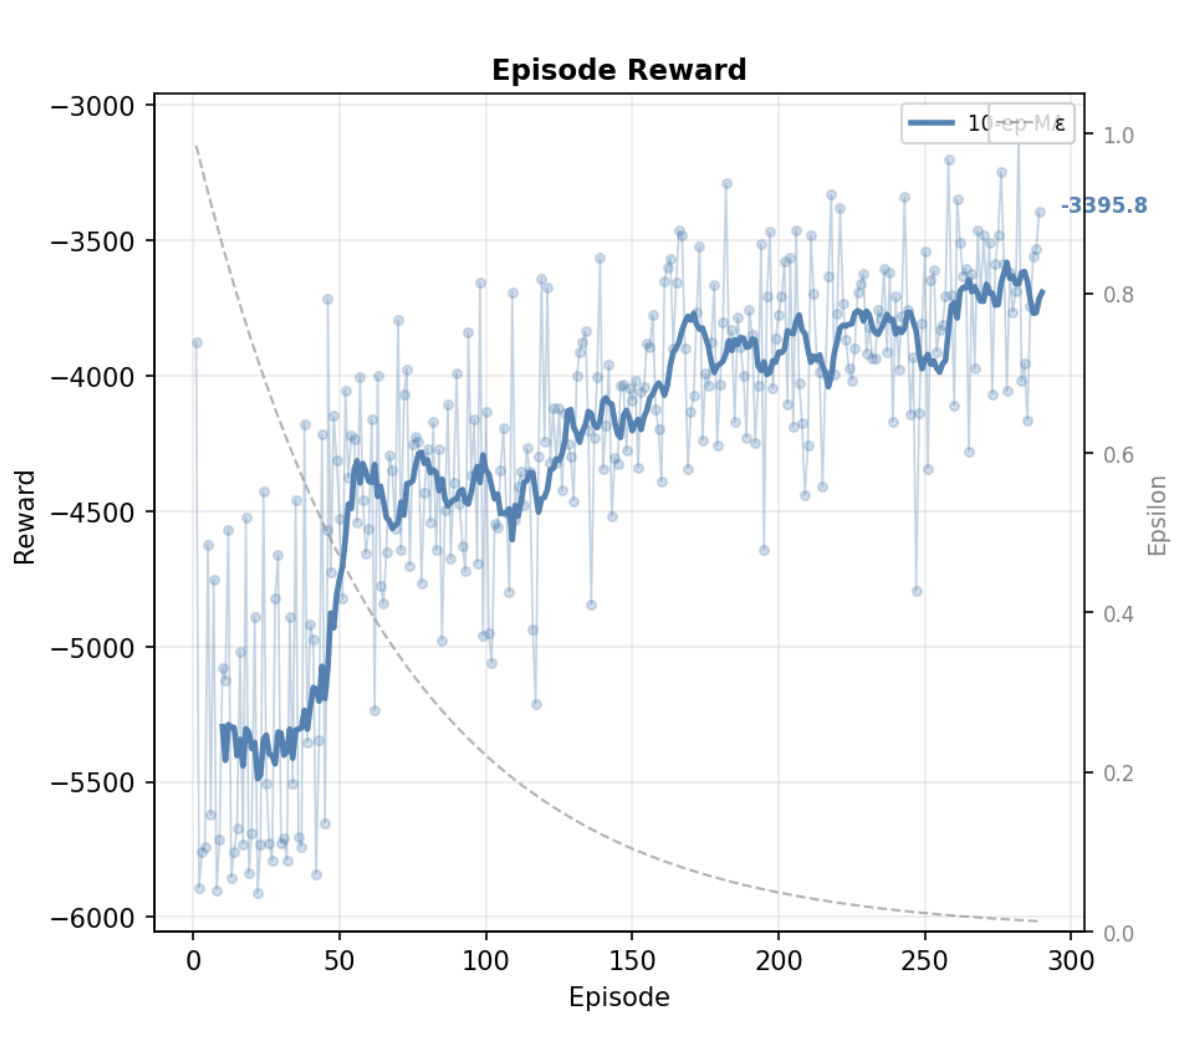
\includegraphics[width=\textwidth]{src/images/figures/reward_function.png}
    \caption{Episode Reward and Epsilon Decay over 300 Training Episodes}
    \label{fig:reward_function}
\end{figure}

\section{Wait Time Reduction Analysis}
\label{sec:wait_time_reduction}

Figure \ref{fig:wait_time} compares hourly average wait times for the Fixed 60s controller and the \gls{dqn} agent (Episode 300) on Day 5. The fixed controller ranges from 29s to 50s with high volatility, while the \gls{dqn} consistently stays between 23s and 30s.

\noindent Key results:
\begin{itemize}
    \item Overall average: \textbf{+22.90\%} improvement across all hours
    \item Morning peak average (9--11 AM): \textbf{+8.26\%} improvement
    \item Evening Peak Average (4--6 PM): \textbf{+19.26\%} improvement
\end{itemize}

\begin{figure}[H]
    \centering
    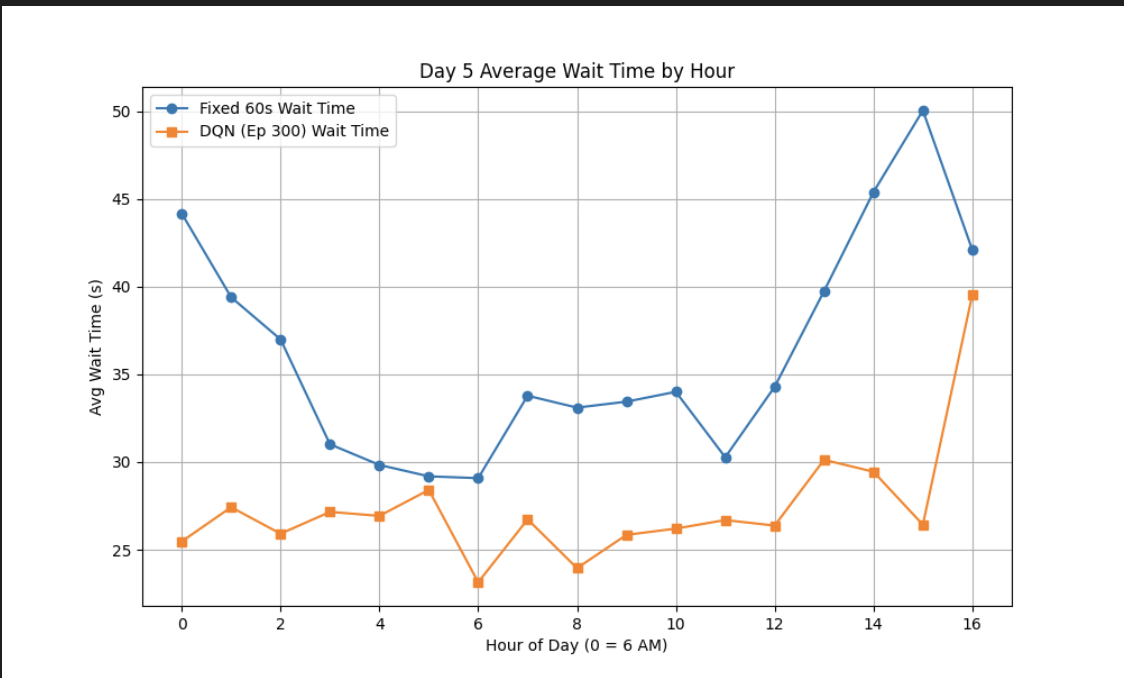
\includegraphics[width=\textwidth]{src/images/figures/wait_time.png}
    \caption{Day 5 Average Wait Time by Hour: Fixed 60s vs DQN (Episode 300)}
    \label{fig:wait_time}
\end{figure}

\section{Queue Length Management Effectiveness}
\label{sec:queue_length_management}

Figure \ref{fig:total_queue} shows hourly average total queue length. The fixed controller sustains 10--13 vehicles throughout peak hours, while the \gls{dqn} holds queues to 5.9--10.3 vehicles. In the evening, the \gls{dqn} clears queues to 1.83 vehicles by 22:00 versus 5.0 for the fixed plan.

\noindent Key results:
\begin{itemize}
    \item Overall average: \textbf{+30.06\%} reduction across all hours
    \item Morning peak average (9--11 AM): \textbf{+21.42\%} improvement
    \item Evening Peak Average (4--6 PM): \textbf{+20.89\%} improvement
\end{itemize}

\begin{figure}[H]
    \centering
    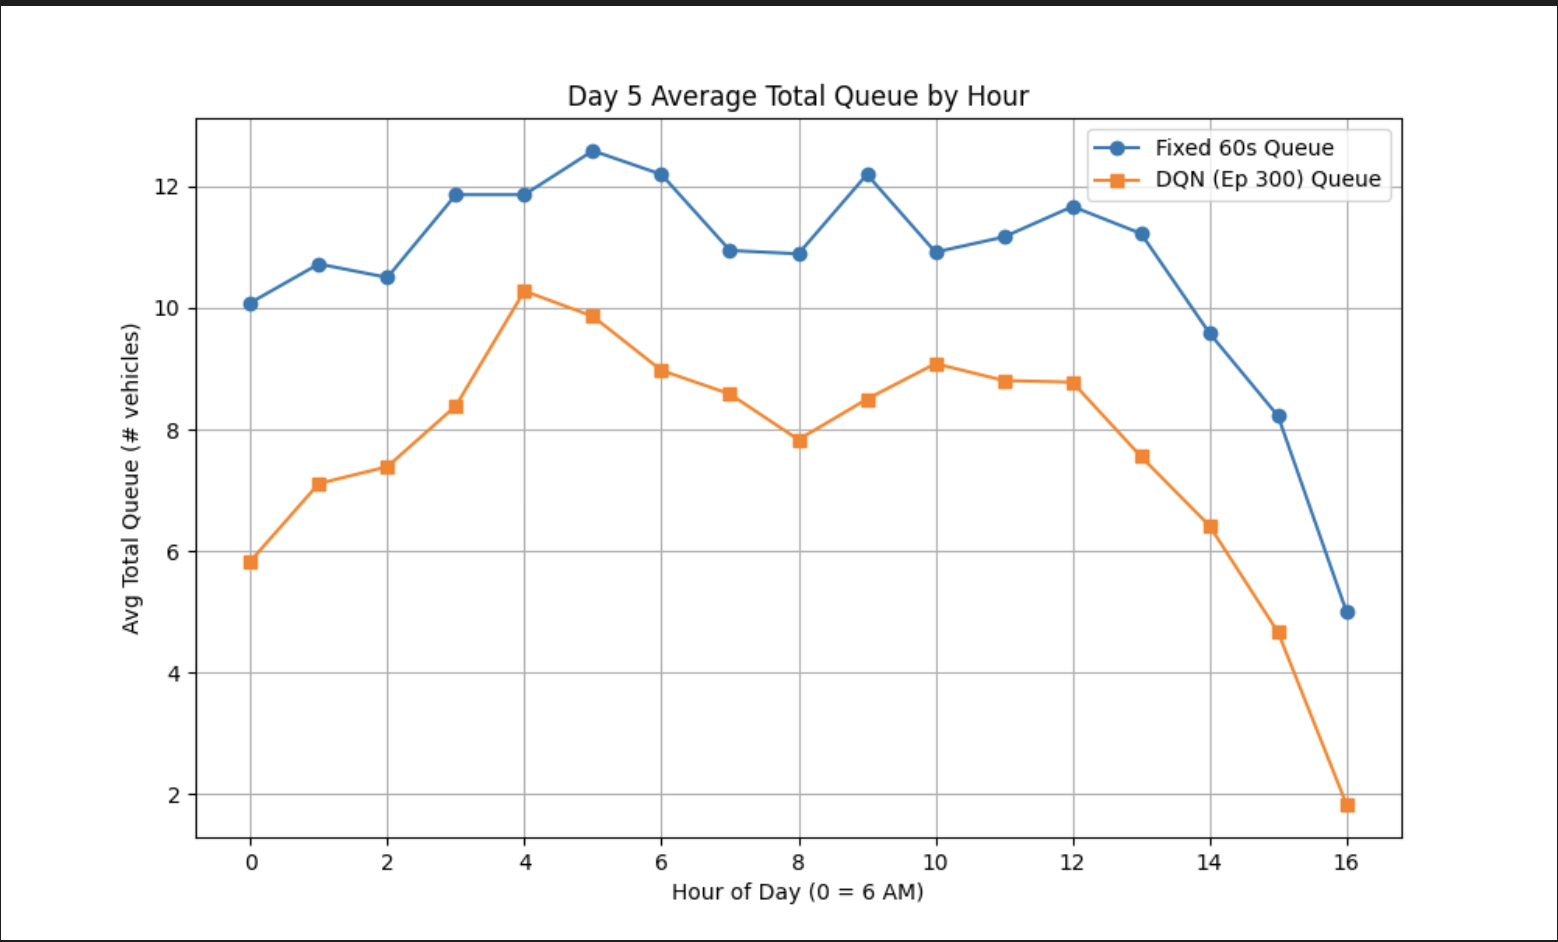
\includegraphics[width=\textwidth]{src/images/figures/total_queue.png}
    \caption{Day 5 Average Total Queue Length by Hour: Fixed 60s vs DQN (Episode 300)}
    \label{fig:total_queue}
\end{figure}

\section{Throughput Efficiency Analysis}
\label{sec:throughput_efficiency}

Figure \ref{fig:throughput_per_second_of_wait_time} shows the throughput efficiency ratio (vehicles per wait-second). The \gls{dqn} curve consistently exceeds the F60 curve at all hours, with the gap widening during peak and off-peak extremes.

\noindent Key results:
\begin{itemize}
    \item Overall average: \textbf{+32.65\%} improvement across all hours
    \item Morning peak average (9--11 AM): \textbf{+9.33\%} improvement
    \item Evening Peak Average (4--6 PM): \textbf{+24.23\%} improvement
\end{itemize}

\begin{figure}[H]
    \centering
    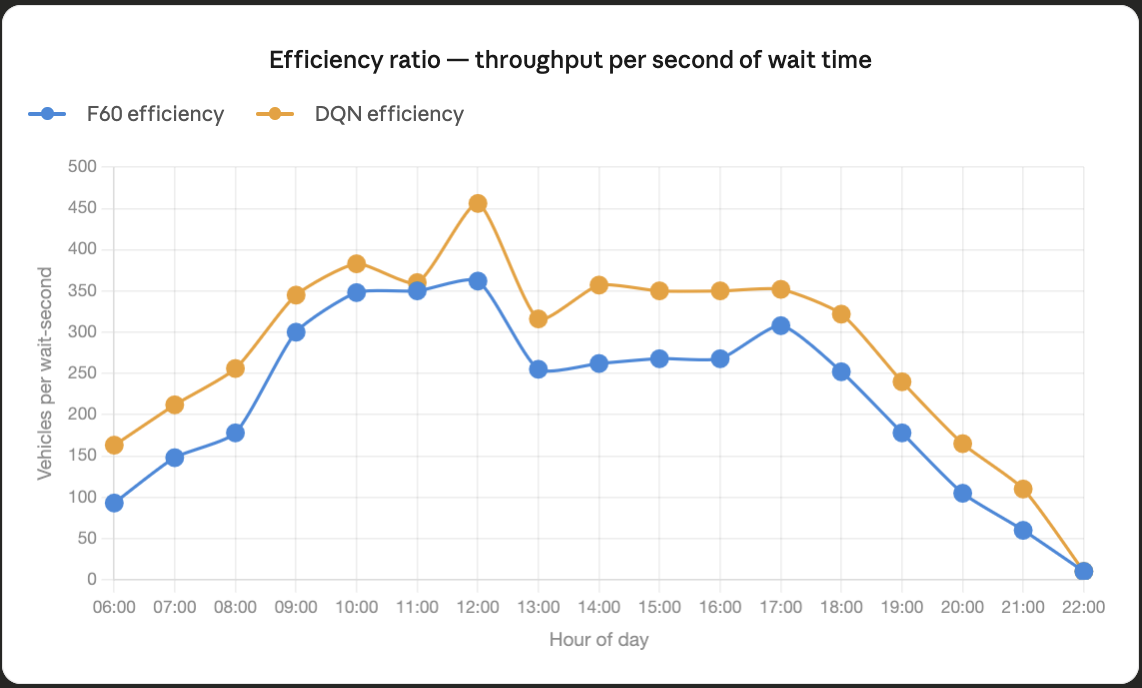
\includegraphics[width=\textwidth]{src/images/figures/throughput_per_second_of_wait_time.png}
    \caption{Efficiency Ratio of Throughput per Second of Wait Time: F60 vs DQN (Episode 300)}
    \label{fig:throughput_per_second_of_wait_time}
\end{figure}

\section{Consolidated Performance Comparison}
\label{sec:consolidated_performance}

Table \ref{tab:wait_queue_comparison} summarises the hour-by-hour comparison. The DQN controller performs better than the fixed-time controller for the reported metrics, but the size of the gain changes noticeably across the day.


\begin{table}[H]
\centering
\caption{Hour-by-Hour Performance: Wait Time and Queue Length (Episode 300)}
\label{tab:wait_queue_comparison}
\small
\begin{tabular}{|c|c|c|c|c|c|}
\hline
\textbf{Time} & \textbf{Wait time (s)} & \textbf{Wait time (s)} & \textbf{Improvement} & \textbf{Queue length (veh)} & \textbf{Queue length (veh)} \\
 & \textbf{Fixed} & \textbf{Imp. Queue} & \textbf{(\%)} & \textbf{Fixed} & \textbf{Imp. Queue} \\
\hline
06:00 & 44.16 & 25.48 & 42.30\% & 10.08 & 5.83 \\
07:00 & 39.39 & 27.43 & 30.37\% & 10.72 & 7.11 \\
08:00 & 36.99 & 25.92 & 29.93\% & 10.50 & 7.39 \\
09:00 & 31.01 & 27.16 & 12.42\% & 11.86 & 8.39 \\
10:00 & 29.84 & 26.93 & 9.73\% & 11.86 & 10.28 \\
11:00 & 29.19 & 28.41 & 2.65\% & 12.58 & 9.86 \\
12:00 & 29.08 & 23.15 & 20.40\% & 12.19 & 8.97 \\
13:00 & 33.78 & 26.74 & 20.85\% & 10.94 & 8.58 \\
14:00 & 33.10 & 23.96 & 27.63\% & 10.89 & 7.83 \\
15:00 & 33.44 & 25.85 & 22.70\% & 12.19 & 8.50 \\
16:00 & 34.00 & 26.21 & 22.92\% & 10.92 & 9.08 \\
17:00 & 30.27 & 26.69 & 11.82\% & 11.17 & 8.81 \\
18:00 & 34.29 & 26.38 & 23.06\% & 11.67 & 8.78 \\
19:00 & 39.74 & 30.13 & 24.18\% & 11.22 & 7.56 \\
20:00 & 45.38 & 29.45 & 35.11\% & 9.58 & 6.42 \\
21:00 & 50.03 & 26.43 & 47.17\% & 8.22 & 4.67 \\
22:00 & 42.09 & 39.53 & 6.10\% & 5.00 & 1.83 \\
\hline
\multicolumn{6}{|c|}{\textit{Overall Average Improvement: Wait Time +22.90\%, Queue Length +30.06\%}} \\
\hline
\end{tabular}
\end{table}

\begin{table}[H]
\centering
\caption{Hour-by-Hour Performance: Throughput Efficiency (Episode 300)}
\label{tab:throughput_comparison}
\small
\begin{tabular}{|c|c|c|}
\hline
\textbf{Time} & \textbf{Throughput efficiency (veh/wait-s)} & \textbf{Throughput efficiency (veh/wait-s)} \\
 & \textbf{Fixed} & \textbf{Imp. Queue} \\
\hline
06:00 & 93 & 163 \\
07:00 & 148 & 212 \\
08:00 & 178 & 256 \\
09:00 & 300 & 345 \\
10:00 & 348 & 383 \\
11:00 & 350 & 360 \\
12:00 & 362 & 456 \\
13:00 & 255 & 316 \\
14:00 & 262 & 357 \\
15:00 & 268 & 350 \\
16:00 & 268 & 350 \\
17:00 & 308 & 352 \\
18:00 & 252 & 322 \\
19:00 & 178 & 240 \\
20:00 & 105 & 165 \\
21:00 & 60 & 110 \\
22:00 & 10 & 10 \\
\hline
\multicolumn{3}{|c|}{\textit{Overall Average Improvement: +32.65\%}} \\
\hline
\end{tabular}
\end{table}



\section{Overall Performance Summary and Analysis}
\label{sec:overall_performance_summary}

The three metrics evaluated - average wait time, average queue length,
and throughput efficiency ratio - collectively present a consistent and
unambiguous picture: the DQN agent outperforms the fixed 60-second
controller across every hour of the simulation day and across every
dimension of traffic performance.

\subsection{Consistency Across Metrics}
\label{subsec:consistency_across_metrics}

The three metrics move in the same direction, which is important for
interpreting the result. A controller can sometimes reduce waiting time
on one approach by shifting delay to another approach. That pattern was
not observed in the Day 5 evaluation: average waiting time, queue length,
and throughput efficiency all improved under the DQN policy. This does
not prove that the policy is optimal, but it does show that the reported
gain is not caused by improving one metric while clearly damaging
another.

\subsection{Throughput Efficiency Ratio Analysis}
\label{subsec:throughput_efficiency_ratio_analysis}

Figure 6-5 compares vehicles processed per second of cumulative wait
time. The DQN curve stays above the fixed 60-second plan throughout the
day. The overall improvement is 32.65\%, which is the largest percentage
gain among the three reported metrics.

The result is useful because total vehicle throughput remained broadly
comparable between the two controllers. In other words, the DQN policy
did not simply push more vehicles into the network; it moved similar
demand with less accumulated delay. The morning peak improvement was
9.33\%, while the evening peak improvement was 24.23\%. This matches the
wait-time and queue-length pattern, where the evening demand gave the
adaptive controller more opportunity to differ from the fixed plan.

\subsection{Peak Hour Behaviour}
\label{subsec:peak_hour_behaviour}

The morning and evening peaks did not behave the same way. From 9-11 AM,
the DQN improvement was 8.26\% for wait time, 21.42\% for queue length,
and 9.33\% for throughput efficiency. From 4-6 PM, the corresponding
improvements were 19.26\%, 20.89\%, and 24.23\%.

This difference is consistent with the reward design. The Max-Pressure
term responds to imbalance between approaches. When the evening demand is
more uneven, the controller has more useful decisions to make. When the
morning demand is closer to saturation across several approaches at once,
there is less spare green time to reallocate.

\subsection{Variance Reduction}
\label{subsec:variance_reduction}

The fixed controller produced a wider range of hourly wait times, from
29s to 50s. The DQN policy stayed within 23-30s for most hours. Queue
lengths show the same pattern: the fixed plan held roughly 10-13 vehicles
during peak periods, while DQN stayed around 5.9-10.3.

This matters because average values alone can hide unstable operation.
For a commuter, a controller with fewer extreme delay periods is more
useful than one that performs well only in short bursts. The smoother
throughput-efficiency curve suggests that the DQN policy reduced those
large swings in delay.

\subsection{Off-Peak Performance}
\label{subsec:off_peak_performance}

The off-peak result shows why fixed timing is inefficient when demand is
low. By 22:00, the average queue length under DQN was 1.83 vehicles,
compared with 5.0 under the fixed plan. The largest hourly wait-time
improvement, 47.17\%, occurred at 21:00.

At those hours, the benefit is not mainly from handling heavy congestion.
It comes from avoiding unnecessary red time when arrivals are sparse. A
fixed cycle keeps serving phases according to schedule even if the active
movement has little traffic. The DQN policy can move away from that phase
sooner.

\subsection{Failure Case Analysis}
\label{subsec:failure_case_analysis}

While the DQN agent demonstrated consistent improvement over the fixed
timer across all hours and metrics, several failure cases and structural
limitations were identified that qualify the scope of these results:

\begin{itemize}
\item
  \textbf{Peak-hour saturation:} The most significant failure case
  occurs during 10:00-11:00 where the wait time improvement falls to
  just 2.65\%, indicating that the agent\textquotesingle s adaptive
  advantage essentially disappears when all approaches are
  simultaneously overloaded. This is not an algorithmic failure but an
  infrastructural constraint - the Thapathali intersection operates
  beyond its designed capacity during peak windows and no signal timing
  strategy alone can resolve that.
\item
  \textbf{Reward signal degradation during saturation:} The Max-Pressure
  reward compares stopline PCU against outgoing PCU but stopline lanes
  at Thapathali are short and fill almost instantly during peak hours,
  making the pressure signal nearly constant regardless of what the
  agent does. This reduces the quality of the learning signal precisely
  during the periods where better control would matter most.
\item
  \textbf{Absence of real downstream network modelling:} Random timer
  signals were placed at outgoing lane ends to simulate backspill but
  these were not calibrated to actual neighbouring intersection
  behaviour, meaning the agent may have learned a policy optimised for
  an artificial downstream condition that does not fully reflect
  reality.
\item
  \textbf{Exclusion of non-motorised and multi-modal traffic:} The
  simulation excludes pedestrians, public transport, and non-motorised
  vehicles which are present at the real Thapathali intersection. Their
  omission means the agent operates in a cleaner environment than would
  exist in actual deployment, and real-world performance could differ
  meaningfully from simulation results.
\item
  \textbf{Limited training data diversity:} The training was conducted
  exclusively on four days of observed traffic data, limiting the
  diversity of demand patterns the agent was exposed to. Unusual traffic
  conditions such as accidents, festivals, road closures, or sudden
  demand surges were not represented in training, and the
  agent\textquotesingle s ability to generalise to such scenarios
  remains untested.
\end{itemize}

\subsection{Summary}
\label{subsec:summary}

The results support a narrower conclusion: for the Day 5 demand used in
testing, the DQN policy handled phase changes better than the fixed
60-second plan. The evidence is strongest because the same pattern
appears in all three metrics. Wait time falls, queue length falls, and
throughput per wait second rises.

The result should still be read within the limits of the experiment. The
agent was not tested against accidents, festivals, lane blockage, or
fully calibrated downstream intersections. What the evaluation shows is
that, under the available Thapathali demand data, using the observed
traffic state gives a clear advantage over a fixed cycle.
